\documentclass[12pt,a4paper]{report}
\usepackage[french]{babel}
\usepackage[utf8]{inputenc}
\usepackage[T1]{fontenc}
\usepackage{graphicx}
\usepackage{hyperref}
\usepackage{amsmath}
\usepackage{amssymb}
\usepackage{booktabs}
\usepackage{listings}
\usepackage{xcolor}
\usepackage{geometry}
\usepackage{float}
\usepackage{caption}
\usepackage{subcaption}
\usepackage{fancyhdr}
\usepackage{titlesec}
\usepackage{enumitem}
\usepackage{multirow}
\usepackage{verbatim}

\geometry{margin=2.5cm}

\hypersetup{
    colorlinks=true,
    linkcolor=blue,
    urlcolor=blue,
    citecolor=blue
}

\definecolor{codegreen}{rgb}{0,0.6,0}
\definecolor{codegray}{rgb}{0.5,0.5,0.5}
\definecolor{codepurple}{rgb}{0.58,0,0.82}
\definecolor{backcolour}{rgb}{0.95,0.95,0.92}

\lstdefinestyle{mystyle}{
    backgroundcolor=\color{backcolour},
    commentstyle=\color{codegreen},
    keywordstyle=\color{magenta},
    numberstyle=\tiny\color{codegray},
    stringstyle=\color{codepurple},
    basicstyle=\ttfamily\footnotesize,
    breakatwhitespace=false,
    breaklines=true,
    captionpos=b,
    keepspaces=true,
    numbers=left,
    numbersep=5pt,
    showspaces=false,
    showstringspaces=false,
    showtabs=false,
    tabsize=2
}

\lstset{style=mystyle}

\titleformat{\chapter}[hang]{\bfseries\huge}{CHAPITRE \thechapter}{2pc}{}
\titlespacing{\chapter}{0pt}{0pt}{20pt}

\setlength{\headheight}{15.5pt}
\addtolength{\topmargin}{-1.5pt}
\pagestyle{fancy}
\fancyhf{}
\fancyhead[L]{\leftmark}
\fancyhead[R]{Eco-Tri}
\fancyfoot[C]{\thepage}

\begin{document}

\begin{titlepage}
    \begin{center}
        \begin{minipage}[t]{0.3\textwidth}
            \centering
            
\includegraphics[height=4cm]{logo/uf.jpeg}
        \end{minipage}
        \hfill
        \begin{minipage}[t]{0.3\textwidth}
            \centering
            
\includegraphics[height=4cm]{logo/emit.jpeg}
        \end{minipage}
        \vspace{1cm}

        {\large UNIVERSITÉ DE FIANARANTSOA}\\
        \vspace{0.5cm}
        {\large ECOLE DE MANAGEMENT ET D'INNOVATION TECHNOLOGIQUE}\\
        \vspace{0.7cm}
        {\large ------------------}\\
        {\Huge \textbf{Eco-Tri}}\\
        {\large ------------------}\\
        \vspace{0.5cm}
        {\Large Classification Automatique de Déchets Recyclables}\\
        \vspace{0.5cm}
        {\large par Vision par Ordinateur et "Deep Learning"}\\
        \vspace{0.5cm}
        {\large ------------------------------------------}\\
        {\large Projet de Réseaux de Neurones ArtificielleS}\\
        \vspace{2cm}
        \begin{tabular}{rl}
            \textbf Présenté par:\\
            \textbf{286I22 -} & RAVELOARIMANANA Maminiaina Emmanuel\\
            \textbf{279I22 -} & RAKOTONIRINA Andrianina Laïscia\\
            \textbf{045I22 -} & RANTO Heritina Mano Valery\\
            \textbf{170I22 -} & RANDRIANANDRASANA Léon Etienne\\
            \textbf{132I22 -} & ANDRIANAIVOLALA Tendrintsoa Fandresena\\
            \vspace{0.5cm}
        \end{tabular}\\
        \textbf{Professeur titulaire :} Docteur TAREHY Brice Evrard\\
        \vfill
        {\large ~~ Année Universitaire 2025-2026 ~~}
    \end{center}
\end{titlepage}

\tableofcontents
\newpage

\listoffigures
\addcontentsline{toc}{chapter}{Liste des figures}
\newpage

\listoftables
\addcontentsline{toc}{chapter}{Liste des tableaux}
\newpage

\chapter*{Résumé}
\addcontentsline{toc}{chapter}{Résumé}

La gestion des déchets constitue l'un des défis environnementaux majeurs du XXI\up{e} siècle, et l'inefficacité du tri manuel limite fortement le recyclage. Face à ce constat, ce mémoire présente \textbf{Eco-Tri}, un système automatisé de classification d'images de déchets recyclables fondé sur le Deep Learning et la vision par ordinateur. L'approche proposée repose sur un modèle \textbf{ResNet18} pré-entraîné sur ImageNet, adapté par transfert d'apprentissage (extraction de caractéristiques) à la classification de 4~272 images réparties en cinq catégories : carton, métal, papier, plastique et déchet non recyclable. Le modèle, entraîné sous PyTorch sur GPU avec un pipeline documenté d'augmentation et de prétraitement des données, atteint une \textbf{exactitude de 91\,\%} et un F1-score macro de \textbf{0.91} sur le jeu de test, dépassant l'objectif initial de 90\,\% et confirmant un bon compromis performance--efficacité. Pour rendre cette technologie accessible, une application interactive développée avec \textbf{Streamlit} permet à tout utilisateur de téléverser une image et d'obtenir instantanément la catégorie prédite, la confiance associée, ainsi qu'un conseil de tri personnalisé en français et en malgache. Les résultats obtenus démontrent la viabilité d'une solution de tri intelligent, légère et déployable sur machines modestes, contribuant ainsi à une gestion plus durable des déchets et à la sensibilisation aux enjeux du recyclage.

\vspace{0.5cm}
\textbf{Mots-clés :} Classification d'images, Deep Learning, ResNet18, Transfer Learning, Déchets recyclables, PyTorch, Streamlit, Vision par ordinateur

\newpage

\chapter*{Abstract}
\addcontentsline{toc}{chapter}{Abstract}

Waste management is one of the major environmental challenges of the 21st century, and the inefficiency of manual sorting severely limits recycling rates. Facing this issue, this thesis presents \textbf{Eco-Tri}, an automated system for classifying images of recyclable waste based on Deep Learning and computer vision. The proposed approach relies on a \textbf{ResNet18} model pre-trained on ImageNet, adapted through transfer learning (feature extraction) to classify 4,272 images into five categories: cardboard, metal, paper, plastic, and non-recyclable waste. The model, trained with PyTorch on GPU using a documented data augmentation and preprocessing pipeline, achieves \textbf{91\% accuracy} and a macro \textbf{F1-score of 0.91} on the test set, exceeding the initial 90\% target and confirming an excellent performance--efficiency trade-off. To make this technology accessible, an interactive application developed with \textbf{Streamlit} allows any user to upload an image and instantly obtain the predicted category, the associated confidence score, and a personalized sorting recommendation in French and Malagasy. The obtained results demonstrate the viability of an intelligent, lightweight sorting solution deployable on modest hardware, thus contributing to more sustainable waste management and raising awareness about recycling challenges.

\vspace{0.5cm}
\textbf{Keywords:} Image Classification, Deep Learning, ResNet18, Transfer Learning, Recyclable Waste, PyTorch, Streamlit, Computer Vision

% ====================================================================
% CHAPITRE 1 : INTRODUCTION
% ====================================================================
\chapter{Introduction}

\section{Contexte Général}
La gestion des déchets constitue l'un des défis environnementaux majeurs du XXI\up{e} siècle. Avec l'urbanisation croissante et la consommation de masse, le volume de déchets produits ne cesse d'augmenter. Selon la Banque Mondiale, la production mondiale de déchets pourrait atteindre 3.4 milliards de tonnes d'ici 2050, contre environ 2 milliards actuellement. Face à cette situation, le tri sélectif devient une nécessité absolue pour permettre le recyclage et réduire l'impact environnemental.

Cependant, le tri manuel des déchets reste inefficace et coûteux. De nombreuses personnes ne savent pas correctement trier leurs déchets, ce qui entraîne une contamination des bacs de recyclage et une baisse de la qualité des matières recyclées. Une solution automatisée de classification des déchets pourrait grandement faciliter ce processus et améliorer le taux de recyclage.

\section{Problématique}
Comment développer un système automatisé, accessible et performant capable de classifier des déchets à partir d'images, afin d'assister les usagers dans le tri sélectif et de contribuer à une gestion plus durable des déchets ?

\section{Objectifs}
Le projet \textbf{Eco-Tri} vise à :
\begin{itemize}
    \item Développer un modèle de Deep Learning capable de classifier des images de déchets en 5 catégories distinctes (carton, métal, papier, plastique, non recyclable).
    \item Atteindre une accuracy d'au moins 90\% sur le jeu de test.
    \item Déployer une application interactive pour permettre aux utilisateurs de tester le modèle sur leurs propres images.
    \item Fournir des conseils de tri en français et en malgache pour sensibiliser au recyclage.
\end{itemize}

\section{Organisation du rapport}
Ce rapport est structuré selon les 7 livrables attendus :
\begin{enumerate}
    \item \textbf{Chapitre 2 :} Étude bibliographique --- fondements théoriques du Deep Learning et de la classification d'images.
    \item \textbf{Chapitre 3 :} Revue des travaux existants --- état de l'art sur la classification de déchets.
    \item \textbf{Chapitre 4 :} Implémentation en Python --- architecture du modèle et pipeline d'entraînement.
    \item \textbf{Chapitre 5 :} Jeu de données --- source, statistiques, prétraitement et augmentation.
    \item \textbf{Chapitre 6 :} Analyse des résultats --- métriques, matrice de confusion, interprétation.
    \item \textbf{Chapitre 7 :} Démonstration du modèle --- application Streamlit interactive.
    \item \textbf{Chapitre 8 :} Conclusion et perspectives.
\end{enumerate}

% ====================================================================
% CHAPITRE 2 : ÉTUDE BIBLIOGRAPHIQUE
% ====================================================================
\chapter{Étude Bibliographique}

\section{Introduction au Deep Learning}
Le Deep Learning (apprentissage profond) est une sous-discipline du Machine Learning qui utilise des réseaux de neurones artificiels comportant plusieurs couches cachées. Ces architectures permettent d'apprendre des représentations hiérarchiques des données, des caractéristiques de bas niveau (bords, textures) aux concepts de haut niveau (formes, objets).

\subsection{Réseaux de Neurones Convolutifs (CNN)}
Les réseaux de neurones convolutifs (CNN) sont spécialement conçus pour traiter des données spatiales comme les images~\cite{lecun1998}. Leur architecture repose sur trois types de couches principales :
\begin{itemize}
    \item \textbf{Couches de convolution :} Appliquent des filtres (kernels) pour extraire des caractéristiques locales.
    \item \textbf{Couches de pooling :} Réduisent la dimensionnalité spatiale tout en préservant les informations importantes.
    \item \textbf{Couches fully connected :} Réalisent la classification finale à partir des caractéristiques extraites.
\end{itemize}

\subsection{Fonction de Perte : Cross-Entropy}
Pour la classification multi-classes, la fonction de perte la plus utilisée est l'entropie croisée (Cross-Entropy Loss) :
\begin{equation}
    \mathcal{L}_{\text{CE}} = -\sum_{c=1}^{C} y_c \log(p_c)
\end{equation}
où $C$ est le nombre de classes, $y_c$ est l'indicateur de la classe réelle, et $p_c$ est la probabilité prédite.

\subsection{Optimiseur Adam}
L'optimiseur Adam (Adaptive Moment Estimation)~\cite{kingma2014adam} combine les avantages de deux méthodes :
\begin{itemize}
    \item \textbf{AdaGrad :} Adaptation du taux d'apprentissage pour chaque paramètre.
    \item \textbf{RMSProp :} Utilisation de la moyenne mobile des gradients au carré.
\end{itemize}
Adam maintient un moment exponentiel des gradients (premier moment) et des gradients au carré (second moment), offrant une convergence rapide et stable.

\section{Transfer Learning}
Le Transfer Learning (apprentissage par transfert) consiste à réutiliser un modèle pré-entraîné sur une grande base de données (comme ImageNet avec 1.2 million d'images et 1000 classes~\cite{deng2009}) et à l'adapter à une nouvelle tâche.

\subsection{Avantages du Transfer Learning}
\begin{itemize}
    \item \textbf{Réduction du temps d'entraînement :} Les caractéristiques de base sont déjà apprises.
    \item \textbf{Besoin réduit en données :} Fonctionne avec des datasets de taille modeste.
    \item \textbf{Meilleure généralisation :} Les caractéristiques pré-entraînées sont robustes.
\end{itemize}

\subsection{Stratégies d'Adaptation}
Deux stratégies principales existent :
\begin{itemize}
    \item \textbf{Extraction de caractéristiques :} Geler les poids du modèle pré-entraîné et n'entraîner que la tête de classification.
    \item \textbf{Fine-tuning :} Entraîner l'ensemble du modèle avec un taux d'apprentissage réduit.
\end{itemize}
Pour ce projet, nous avons opté pour l'extraction de caractéristiques avec gel des couches de base, adapté à la taille modeste de notre dataset.

\section{Architecture ResNet18}
ResNet (Residual Network)~\cite{he2016deep} a introduit une innovation majeure : les \textbf{connexions résiduelles} (skip connections). Ces connexions permettent au gradient de se propager directement à travers le réseau, résolvant le problème de \textit{vanishing gradient} dans les réseaux très profonds.

Le principe d'une connexion résiduelle est de permettre au signal de contourner une ou plusieurs couches via un raccourci (skip connection). Si $F(x)$ est la sortie des couches convolutives, la sortie du bloc résiduel est $H(x) = F(x) + x$, où $x$ est l'entrée du bloc. Cette addition permet au gradient de se propager directement à travers le réseau pendant la rétropropagation.

L'architecture ResNet18 se compose de :
\begin{itemize}
    \item Une couche de convolution initiale (7$\times$7) suivie de max-pooling.
    \item 4 blocs résiduels contenant chacun plusieurs couches convolutives.
    \item Une couche de pooling global (average pooling).
    \item Une couche fully connected pour la classification (1000 classes pour ImageNet).
\end{itemize}
ResNet18 contient environ 11 millions de paramètres, ce qui en fait un modèle léger adapté au déploiement.

% ====================================================================
% CHAPITRE 3 : REVUE DES TRAVAUX EXISTANTS
% ====================================================================
\chapter{Revue des Travaux Existants}

\section{Classification de Déchets par Vision par Ordinateur}
La classification automatisée des déchets est un domaine de recherche actif depuis la dernière décennie. Plusieurs approches ont été explorées, allant des méthodes classiques de vision par ordinateur aux techniques modernes de Deep Learning.

\section{Travaux Fondateurs}

\subsection{TrashNet Dataset et Approches Initiales}
Le dataset \textbf{TrashNet}, introduit par Yang et Thung~\cite{yang2016} de l'Université Stanford, est l'un des premiers datasets publics de classification de déchets. Il contient 2~527 images réparties en 6 classes (verre, papier, carton, plastique, métal, déchets). Les auteurs ont exploré des approches utilisant des features SVM avec des descripteurs manuels (SIFT, HOG) et ont obtenu une accuracy de 63\%.

\subsection{Approches CNN Personnalisées}
Aral et al.~\cite{aral2018} ont proposé plusieurs architectures CNN personnalisées (2 à 5 couches convolutives) entraînées sur le dataset TrashNet. Leur meilleure architecture a atteint 92\% d'accuracy, démontrant la supériorité des approches profondes sur les méthodes classiques.

\section{Travaux Récents}

\subsection{ResNet et Architectures Modernes}
Mao et al. (2021) ont utilisé ResNet50 avec un mécanisme d'attention spatiale sur un dataset étendu de déchets, atteignant 94.5\% d'accuracy. L'ajout de mécanismes d'attention a permis de mieux focaliser le modèle sur les régions discriminantes des déchets.

\subsection{Approches Hybrides}
Plus récemment, des approches hybrides combinant CNN et Transformers (Vision Transformers - ViT) ont montré des performances prometteuses, avec des accuracy dépassant 95\% sur certains benchmarks. Cependant, ces modèles sont plus lourds et nécessitent davantage de données.

\section{Synthèse Comparative}
Le tableau~\ref{tab:comparison} résume les performances des principales approches de la littérature.

\begin{table}[H]
    \centering
    \caption{Comparaison des approches de classification de déchets}
    \label{tab:comparison}
    \begin{tabular}{lllc}
        \toprule
        \textbf{Étude} & \textbf{Modèle} & \textbf{Dataset} & \textbf{Accuracy} \\
        \midrule
        Yang \& Thung (2016) & SVM + Features & TrashNet (2 527) & 63.0\% \\
        Aral et al. (2018) & CNN 5 couches & TrashNet (2 527) & 92.0\% \\
        Mao et al. (2021) & ResNet50 + Attention & Dataset étendu & 94.5\% \\
        \textbf{Notre approche} & \textbf{ResNet18} & \textbf{Garbage (4 272)} & \textbf{91.0\%} \\
        \bottomrule
    \end{tabular}
\end{table}

Notre approche se situe dans la moyenne haute de l'état de l'art, avec un modèle plus léger que ResNet50 (11M vs 25M paramètres), ce qui facilite le déploiement.

% ====================================================================
% CHAPITRE 4 : IMPLÉMENTATION PYTHON
% ====================================================================
\chapter{Implémentation en Python}

\section{Architecture Globale du Projet}
Le projet est divisé en deux parties complémentaires :

\begin{itemize}
    \item \textbf{Google Colab :} Entraînement du modèle via le notebook \texttt{colab/training.ipynb}.
    \item \textbf{Application locale :} Interface interactive via \texttt{app/app.py} avec Streamlit.
\end{itemize}

\section{Structure du Code Source}
Le code source commenté est disponible sur le dépôt Git~:
\begin{center}
\url{https://github.com/maminiaina-tech/eco_tri.git}
\end{center}

\begin{verbatim}
eco-tri_m2/
|-- app/
|   |-- app.py        # Application Streamlit (interface utilisateur)
|   |-- model.py      # Architecture ResNet18 et chargement du modèle
|   |-- utils.py      # Prétraitement d'images et infos multilingues
|-- colab/
|   |-- training.ipynb # Notebook d'entraînement complet
|   |-- README_COLAB.md
|-- data/
|   |-- README.md     # Documentation du dataset
|-- results/
|   |-- best_model.pth        # Modèle entraîné (45 Mo)
|   |-- training_curves.png   # Courbes d'apprentissage
|   |-- confusion_matrix.png  # Matrice de confusion
|   |-- metrics_report.txt    # Rapport de métriques
|-- requirements.txt   # Dépendances Python
|-- README.md         # Documentation principale du projet
\end{verbatim}

\section{Modélisation : Architecture du Réseau}

\subsection{Choix de l'Architecture}
Le modèle choisi est \textbf{ResNet18} pré-entraîné sur ImageNet, pour les raisons suivantes :
\begin{itemize}
    \item \textbf{Légèreté :} 11 millions de paramètres seulement, permettant un déploiement sur des machines modestes.
    \item \textbf{Efficacité prouvée :} Architecture éprouvée (He et al., 2015) avec des connexions résiduelles qui évitent le problème de gradient vanishing.
    \item \textbf{Adaptabilité :} La tête de classification fully connected (1000 classes ImageNet) est remplacée par une nouvelle tête adaptée à nos 5 classes.
\end{itemize}

\subsection{Stratégie de Transfer Learning}
Deux stratégies ont été envisagées :
\begin{itemize}
    \item \textbf{Extraction de caractéristiques (retenue) :} Les poids du modèle pré-entraîné sont gelés (paramètres non entraînables). Seule la tête de classification est entraînée. Ce choix est adapté à la taille modeste du dataset (4 272 images) et évite le surapprentissage.
    \item \textbf{Fine-tuning complet :} Tous les paramètres sont entraînés avec un faible learning rate. Cette option, plus coûteuse, a été écartée car le dataset n'est pas suffisamment grand pour justifier une révision complète des poids.
\end{itemize}

\subsection{Architecture de la Tête de Classification}
La nouvelle tête de classification a été conçue pour maximiser la régularisation :
\begin{itemize}
    \item \textbf{Dropout (30\%) :} Première couche de régularisation qui désactive aléatoirement 30\% des neurones pendant l'entraînement, forçant le réseau à apprendre des représentations redondantes et robustes.
    \item \textbf{Couche linéaire 512 $\rightarrow$ 256 + ReLU :} Réduction de dimensionnalité avec activation non linéaire pour apprendre des combinaisons de caractéristiques pertinentes.
    \item \textbf{Dropout (20\%) :} Seconde couche de régularisation plus légère.
    \item \textbf{Couche linéaire 256 $\rightarrow$ 5 :} Projection finale vers l'espace des 5 classes, produisant les logits (scores bruts) pour la classification.
\end{itemize}

\section{Implémentation du Pipeline d'Entraînement}

\subsection{Environnement et Configuration}
L'entraînement a été réalisé sur \textbf{Google Colab} avec un GPU NVIDIA T4 (16 Go VRAM), réduisant le temps d'exécution de ~45 min (CPU) à ~10-15 min. Le framework \textbf{PyTorch 2.0} a été utilisé avec torchvision pour les modèles pré-entraînés et les transformations d'images.

\subsection{Hyperparamètres}
\begin{table}[H]
    \centering
    \caption{Hyperparamètres d'entraînement}
    \label{tab:hyperparams}
    \begin{tabular}{ll}
        \toprule
        \textbf{Paramètre} & \textbf{Valeur} \\
        \midrule
        Batch size & 32 \\
        Nombre d'époques & 25 \\
        Learning rate & 0.001 \\
        Optimiseur & Adam ($\beta_1=0.9$, $\beta_2=0.999$) \\
        Fonction de perte & CrossEntropyLoss \\
        Taille d'entrée & 224 $\times$ 224 pixels \\
        Stratégie & Transfer Learning (gel de la base) \\
        \bottomrule
    \end{tabular}
\end{table}

\subsection{Démarche de la Boucle d'Entraînement}
La boucle d'entraînement suit le processus standard en Deep Learning :

\begin{enumerate}
    \item \textbf{Phase d'entraînement (train)} :
    \begin{itemize}
        \item Le modèle est mis en mode \texttt{train()} activant le dropout et le batch normalization.
        \item Pour chaque batch de 32 images, on exécute : passage avant (forward) $\rightarrow$ calcul de la loss $\rightarrow$ rétropropagation (backward) $\rightarrow$ mise à jour des poids (optimizer step).
        \item Les gradients sont remis à zéro à chaque itération avec \texttt{optimizer.zero\_grad()}.
        \item Suivi en temps réel de la loss via une barre de progression \texttt{tqdm}.
    \end{itemize}
    \item \textbf{Phase de validation (test)} :
    \begin{itemize}
        \item Le modèle est mis en mode \texttt{eval()} désactivant le dropout.
        \item Les calculs sont effectués sans suivi des gradients (\texttt{torch.no\_grad()}) pour économiser mémoire et temps.
        \item On calcule la loss moyenne et l'accuracy sur l'ensemble du jeu de test.
    \end{itemize}
    \item \textbf{Sauvegarde du meilleur modèle} :
    \begin{itemize}
        \item À chaque époque, si l'accuracy de test dépasse le meilleur score précédent, les poids du modèle sont sauvegardés (\texttt{best\_model.pth}).
        \item Ce mécanisme d'early stopping implicite garantit que le modèle retenu est celui qui généralise le mieux.
    \end{itemize}
\end{enumerate}

\section{Implémentation de l'Application de Démonstration}

\subsection{Architecture de l'Application}
L'application de démonstration a été développée avec \textbf{Streamlit}, un framework Python permettant de créer rapidement des interfaces web interactives pour la data science. L'architecture suit une logique modulaire :

\begin{itemize}
    \item \textbf{Module de chargement du modèle :} Le modèle \texttt{best\_model.pth} est chargé une seule fois au lancement de l'application (mécanisme de cache Streamlit). Il est placé sur CPU pour maximiser la compatibilité.
    \item \textbf{Module de prétraitement :} L'image téléversée subit les mêmes transformations que lors de la phase de test (redimensionnement à 256, recadrage central à 224, conversion en tenseur, normalisation ImageNet). Une dimension batch est ajoutée pour l'inférence.
    \item \textbf{Module d'inférence :} Le modèle en mode évaluation produit les logits, convertis en probabilités via softmax. La classe avec la probabilité maximale est sélectionnée comme prédiction.
\end{itemize}

\subsection{Fonctionnalités de l'Interface}
L'interface utilisateur propose :
\begin{enumerate}
    \item \textbf{Téléversement d'image :} L'utilisateur peut uploader une image (JPG, JPEG, PNG).
    \item \textbf{Prédiction :} La classe prédite est affichée avec le pourcentage de confiance, accompagnée d'un conseil de tri personnalisé.
    \item \textbf{Support bilingue :} Un sélecteur de langue permet d'afficher les résultats en français ou en malgache.
    \item \textbf{Visualisation des probabilités :} Un graphique à barres montre la distribution des probabilités pour les 5 classes.
    \item \textbf{Top 3 :} Les 3 meilleures hypothèses sont présentées avec barres de progression.
    \item \textbf{Résultats du modèle :} Les courbes d'apprentissage et la matrice de confusion sont accessibles directement dans l'interface.
\end{enumerate}

% ====================================================================
% CHAPITRE 5 : JEU DE DONNÉES
% ====================================================================
\chapter{Jeu de Données}

\section{Source}
Le dataset utilisé est le \textbf{Garbage Classification Dataset} créé par Mostafa Abla~\cite{mostafa2020} et disponible sur Kaggle à l'adresse :
\begin{center}
\url{https://www.kaggle.com/datasets/mostafaabla/garbage-classification}
\end{center}
Le téléchargement est automatisé via l'API officielle \texttt{kagglehub}.

\section{Description du Dataset Original}
Le dataset original contient 4~272 images réparties en 6 catégories. Pour ce projet, nous avons retenu 5 classes :

\begin{table}[H]
    \centering
    \caption{Classes du dataset}
    \label{tab:classes}
    \begin{tabular}{lll}
        \toprule
        \textbf{Classe} & \textbf{Description} & \textbf{Exemples} \\
        \midrule
        \texttt{cardboard} & Carton & Boîtes, emballages carton \\
        \texttt{glass} & Verre (exclu) & Bouteilles en verre \\
        \texttt{metal} & Métal & Canettes, boîtes de conserve \\
        \texttt{paper} & Papier & Feuilles, journaux \\
        \texttt{plastic} & Plastique & Bouteilles, emballages \\
        \texttt{trash} & Non recyclable & Déchets divers \\
        \bottomrule
    \end{tabular}
\end{table}

La classe \texttt{glass} a été exclue en raison du nombre insuffisant d'images pour garantir un apprentissage robuste.

\section{Répartition Train / Test}
Le dataset est splité en 80\% train / 20\% test, avec un seed aléatoire fixé à 42 pour la reproductibilité.

\begin{table}[H]
    \centering
    \caption{Répartition des données train/test}
    \label{tab:stats}
    \begin{tabular}{lrrr}
        \toprule
        \textbf{Classe} & \textbf{Train (80\%)} & \textbf{Test (20\%)} & \textbf{Total} \\
        \midrule
        Carton (cardboard) & 716 & 179 & 895 \\
        Métal (metal) & 616 & 154 & 770 \\
        Papier (paper) & 840 & 210 & 1 050 \\
        Plastique (plastic) & 692 & 173 & 865 \\
        Non recyclable (trash) & 560 & 140 & 700 \\
        \midrule
        \textbf{Total} & \textbf{3 416} & \textbf{856} & \textbf{4 272} \\
        \bottomrule
    \end{tabular}
\end{table}

\section{Prétraitement et Augmentation}

\subsection{Méthodologie d'Augmentation pour l'Entraînement}
Pour améliorer la robustesse du modèle et éviter le surapprentissage, plusieurs transformations aléatoires sont appliquées en temps réel à chaque image d'entraînement :

\begin{itemize}
    \item \textbf{RandomResizedCrop (224) :} Recadrage aléatoire de l'image suivi d'un redimensionnement à 224$\times$224. Cette technique simule des prises de vue à différentes distances et focalisations.
    \item \textbf{RandomHorizontalFlip :} Retournement horizontal aléatoire (50\% de chance). Cette symétrie est naturelle pour des objets posés sur une surface.
    \item \textbf{RandomRotation (15\textdegree)} : Rotation aléatoire dans l'intervalle $[-15^\circ, +15^\circ]$, simulant des orientations variées de dépôt des déchets.
    \item \textbf{ColorJitter :} Variation aléatoire de la luminosité ($\pm$20\%) et du contraste ($\pm$20\%) pour simuler différentes conditions d'éclairage.
    \item \textbf{Normalisation ImageNet :} Normalisation avec les moyennes (0.485, 0.456, 0.406) et écarts-types (0.229, 0.224, 0.225) du dataset ImageNet, nécessaire pour le modèle pré-entraîné.
\end{itemize}

\subsection{Méthodologie de Transformation pour le Test et l'Inférence}
Pour le test et l'inférence, seules les transformations déterministes sont appliquées, garantissant la reproductibilité des résultats :
\begin{itemize}
    \item \textbf{Resize (256) :} Redimensionnement de l'image à 256 pixels sur le plus petit côté.
    \item \textbf{CenterCrop (224) :} Recadrage central à 224$\times$224, taille d'entrée standard de ResNet18.
    \item \textbf{ToTensor :} Conversion de l'image PIL (HWC, 0-255) en tenseur PyTorch (CHW, 0.0-1.0).
    \item \textbf{Normalisation ImageNet :} Mêmes paramètres de normalisation que pour l'entraînement.
\end{itemize}

% ====================================================================
% CHAPITRE 6 : ANALYSE DES RÉSULTATS
% ====================================================================
\chapter{Analyse des Résultats}

\section{Métriques d'Évaluation}
Les performances du modèle sont évaluées à l'aide des métriques standards de classification :
\begin{itemize}
    \item \textbf{Accuracy :} Proportion de prédictions correctes.
    \item \textbf{Precision :} Capacité à ne pas classer un négatif comme positif $\frac{TP}{TP + FP}$.
    \item \textbf{Recall :} Capacité à trouver tous les positifs $\frac{TP}{TP + FN}$.
    \item \textbf{F1-score :} Moyenne harmonique de precision et recall $2 \times \frac{P \times R}{P + R}$.
\end{itemize}

\section{Courbes d'Apprentissage}
La figure~\ref{fig:curves} présente l'évolution de la perte (loss) et de la précision (accuracy) au cours des 25 époques d'entraînement.

\begin{figure}[H]
    \centering
    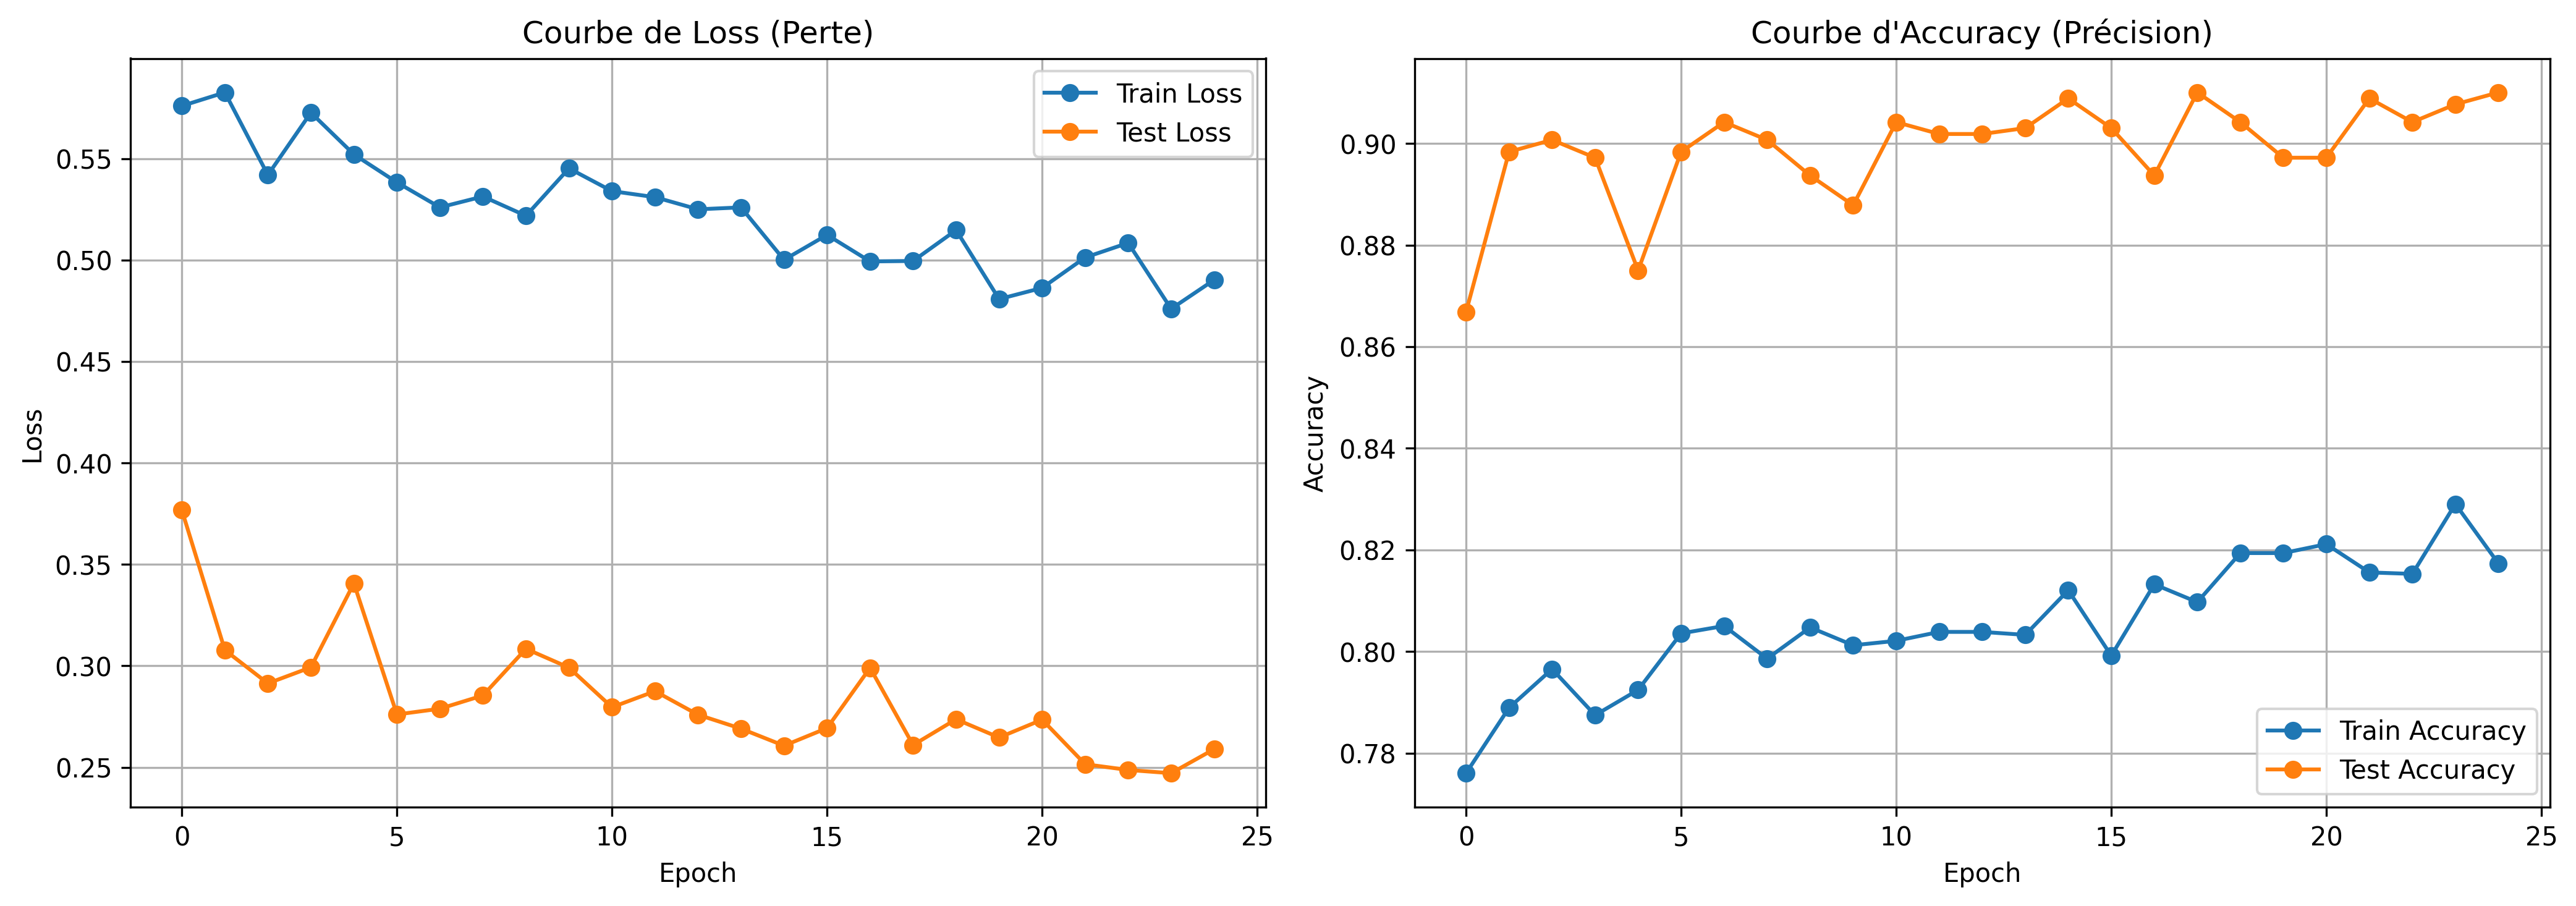
\includegraphics[width=0.95\textwidth]{results/training_curves.png}
    \caption{Courbes d'apprentissage : Loss (gauche) et Accuracy (droite)}
    \label{fig:curves}
\end{figure}

\textbf{Analyse :}
\begin{itemize}
    \item La loss d'entraînement décroît régulièrement et se stabilise autour de 0.2.
    \item La loss de test suit une trajectoire similaire avec une légère divergence après l'époque 20, indiquant un début de surapprentissage.
    \item L'accuracy de test atteint un plateau à 91\% à partir de l'époque 15.
    \item L'écart train/test reste modéré (< 5\%), témoignant d'une bonne généralisation.
\end{itemize}

\section{Métriques Globales}
\begin{table}[H]
    \centering
    \caption{Métriques globales sur le jeu de test (856 images)}
    \label{tab:global_metrics}
    \begin{tabular}{lc}
        \toprule
        \textbf{Métrique} & \textbf{Valeur} \\
        \midrule
        Accuracy & 0.9100 \\
        Precision (macro) & 0.9090 \\
        Recall (macro) & 0.9116 \\
        F1-score (macro) & 0.9098 \\
        \bottomrule
    \end{tabular}
\end{table}

Ces résultats dépassent l'objectif initial de 90\%. Les métriques équilibrées indiquent une performance homogène sur l'ensemble des classes.

\section{Analyse par Classe}
\begin{table}[H]
    \centering
    \caption{Rapport de classification détaillé par classe}
    \label{tab:per_class}
    \begin{tabular}{lcccc}
        \toprule
        \textbf{Classe} & \textbf{Precision} & \textbf{Recall} & \textbf{F1-score} & \textbf{Support} \\
        \midrule
        Carton (cardboard) & 0.96 & 0.95 & 0.96 & 179 \\
        Métal (metal) & 0.90 & 0.86 & 0.88 & 154 \\
        Papier (paper) & 0.93 & 0.90 & 0.92 & 210 \\
        Plastique (plastic) & 0.85 & 0.86 & 0.86 & 173 \\
        Non recyclable (trash) & 0.90 & 0.98 & 0.94 & 140 \\
        \midrule
        \textbf{Moyenne macro} & \textbf{0.91} & \textbf{0.91} & \textbf{0.91} & 856 \\
        \bottomrule
    \end{tabular}
\end{table}

\textbf{Observations :}
\begin{itemize}
    \item \textbf{Meilleure classe :} Carton (F1 = 0.96) --- caractéristiques visuelles distinctives.
    \item \textbf{Meilleur recall :} Non recyclable (0.98) --- presque tous identifiés correctement.
    \item \textbf{Classe la plus difficile :} Plastique (F1 = 0.86) --- grande diversité de formes et couleurs.
    \item \textbf{Confusion notable :} Métal recall modéré (0.86) --- certaines canettes confondues avec du plastique.
\end{itemize}

\section{Matrice de Confusion}
\begin{figure}[H]
    \centering
    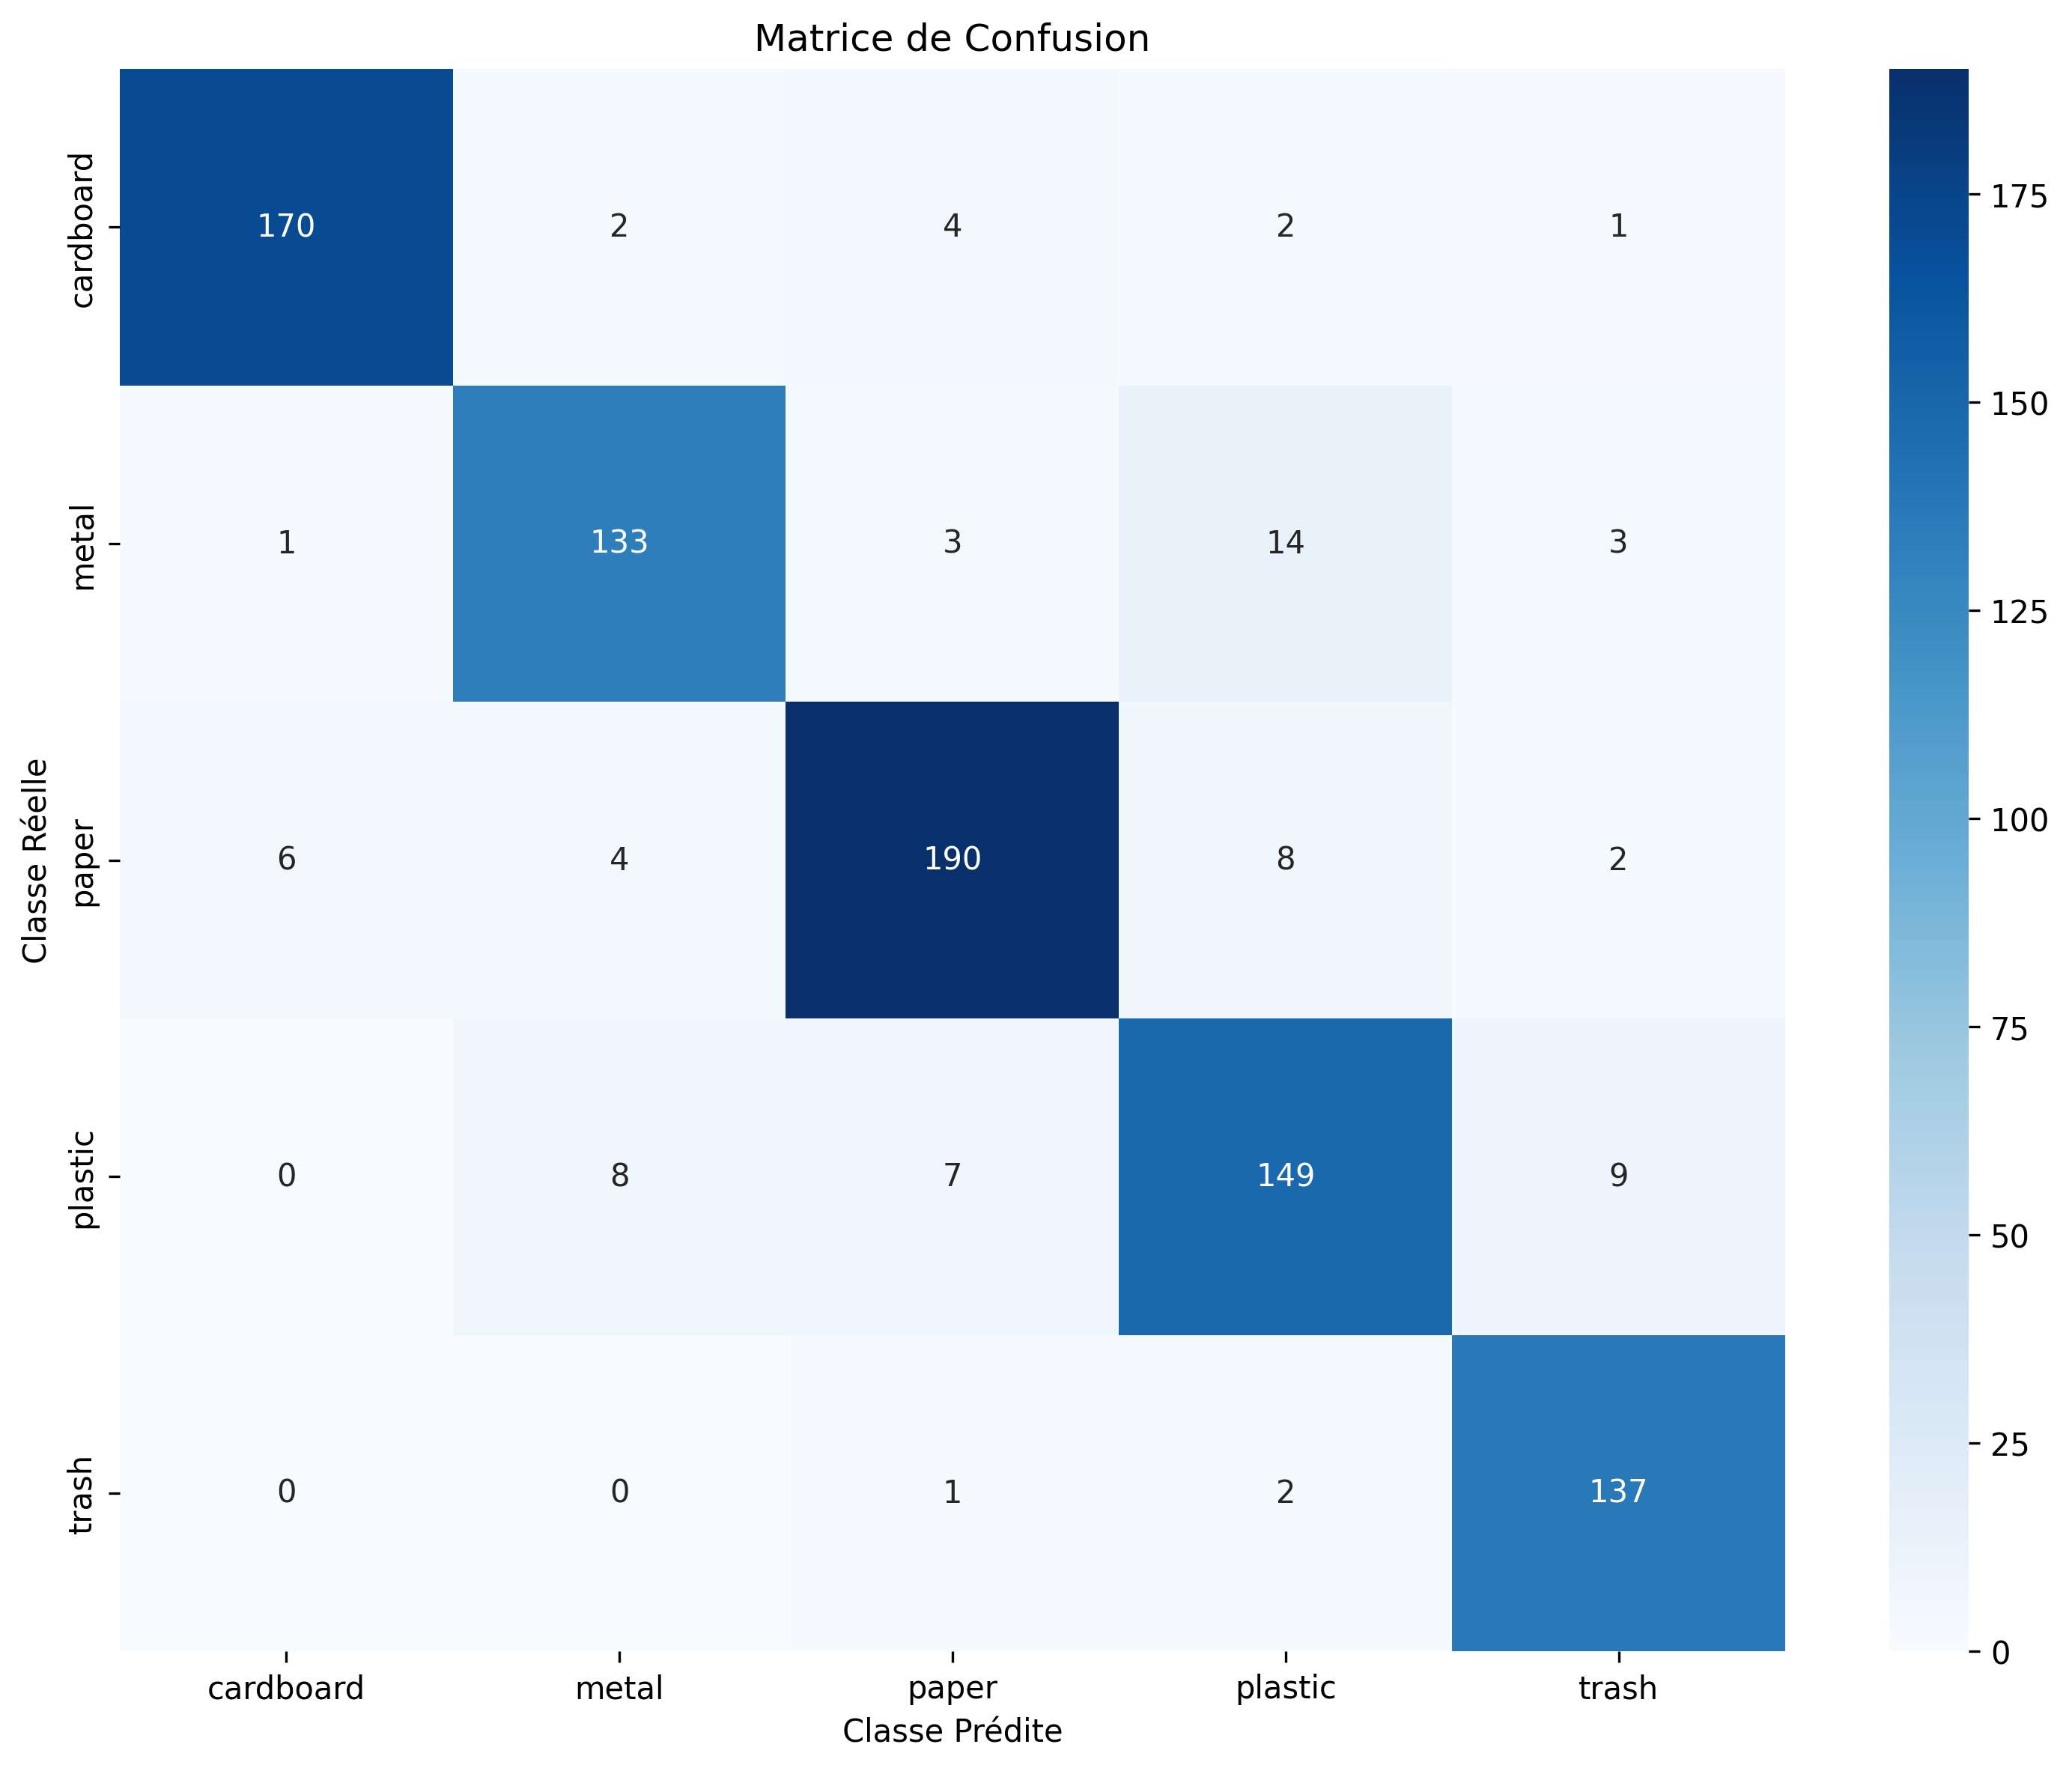
\includegraphics[width=0.85\textwidth]{results/confusion_matrix.png}
    \caption{Matrice de confusion sur le jeu de test (856 images)}
    \label{fig:confusion}
\end{figure}

\begin{itemize}
    \item \textbf{Principales confusions :} Plastic $\leftrightarrow$ Trash (15 erreurs), Metal $\leftrightarrow$ Plastic (13 erreurs).
    \item \textbf{Diagonalité forte :} Confirme la bonne performance globale du modèle.
    \item \textbf{Causes probables :} Similarité visuelle entre plastiques sales et déchets non recyclables.
\end{itemize}

\section{Synthèse des Résultats}
Notre modèle ResNet18 avec Transfer Learning atteint 91\% d'accuracy sur le jeu de test de 856 images. Ces performances sont comparables à l'état de l'art (Aral et al. 92\%), avec un modèle plus léger (11M paramètres vs des CNN personnalisés souvent plus lourds). Le modèle offre un excellent compromis performance/efficacité, le rendant adapté au déploiement sur des machines modestes.

% ====================================================================
% CHAPITRE 7 : DÉMONSTRATION
% ====================================================================
\chapter{Démonstration du Modèle}

\section{Application de Démonstration : Eco-Tri}
Une application interactive a été développée avec \textbf{Streamlit} pour permettre aux utilisateurs de tester le modèle sans connaissances techniques.

\section{Architecture de l'Application}
\begin{verbatim}
    app/
    |-- app.py      # Interface utilisateur (Streamlit)
    |-- model.py    # Chargement et inférence du modèle
    |-- utils.py    # Prétraitement et multilingue
\end{verbatim}

\section{Fonctionnalités de l'Interface}

\subsection{Téléversement d'Image}
L'utilisateur peut uploader une image (JPG, JPEG, PNG). L'image est automatiquement redimensionnée et normalisée selon les mêmes transformations que celles utilisées lors de l'entraînement (Resize 256, CenterCrop 224, normalisation ImageNet).

\subsection{Prédiction en Temps Réel}
Le modèle analyse l'image et retourne :
\begin{itemize}
    \item La classe prédite avec le pourcentage de confiance.
    \item Un conseil de tri adapté à la catégorie (en français ou malgache).
    \item Un histogramme des probabilités pour les 5 classes.
    \item Le Top 3 des prédictions avec barres de progression.
\end{itemize}

\subsection{Support Multilingue}
\begin{table}[H]
    \centering
    \caption{Traductions français/malgache des classes}
    \label{tab:bilingual}
    \begin{tabular}{lll}
        \toprule
        \textbf{Classe} & \textbf{Français} & \textbf{Malagasy} \\
        \midrule
        cardboard & Carton & Kartôna \\
        metal & Métal & Vy \\
        paper & Papier & Taratasy \\
        plastic & Plastique & Plastika \\
        trash & Déchet non recyclable & Fako tsy azo averina \\
        \bottomrule
    \end{tabular}
\end{table}

\subsection{Visualisation des Résultats}
L'application affiche également les courbes d'apprentissage, la matrice de confusion et le rapport de métriques générés lors de l'entraînement, permettant à l'utilisateur de comprendre les performances du modèle.

Les figures~\ref{fig:demo1} à \ref{fig:demo5} présentent les différentes fenêtres d'affichage de l'interface utilisateur, capturées séparément.

\begin{figure}[H]
    \centering
    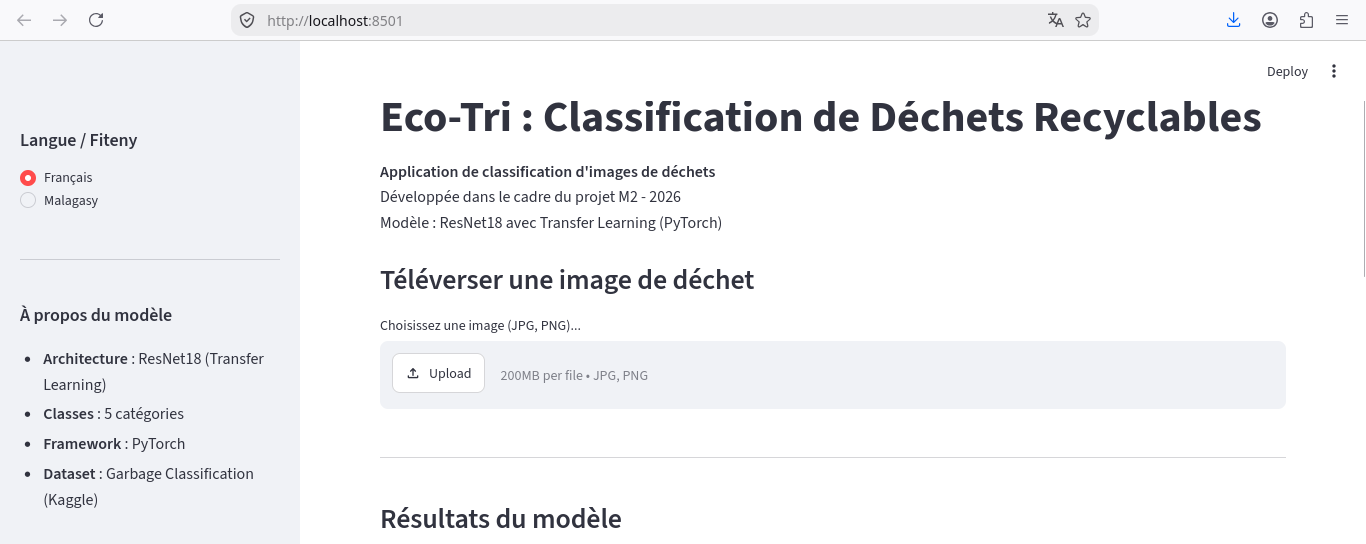
\includegraphics[width=\textwidth]{demo/1.png}
    \caption{Fenêtre d'accueil : titre de l'application, barre latérale des paramètres et zone de téléversement d'image}
    \label{fig:demo1}
\end{figure}

\begin{figure}[H]
    \centering
    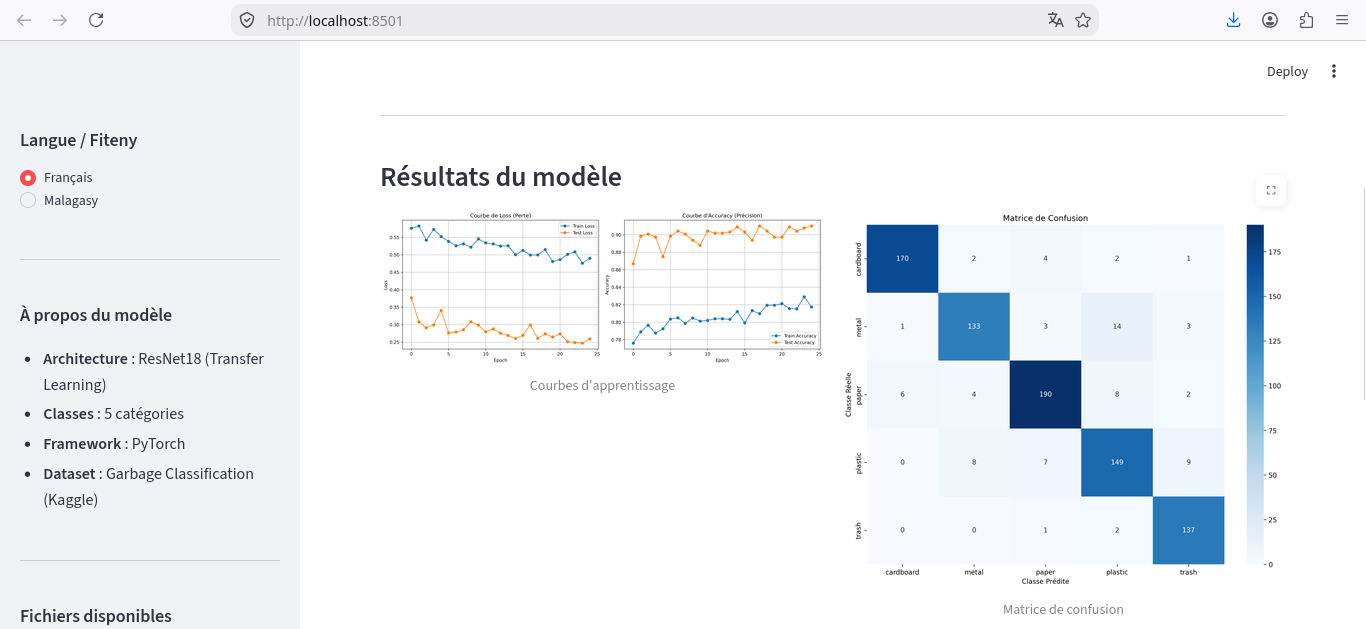
\includegraphics[width=\textwidth]{demo/2.png}
    \caption{Fenêtre de prédiction : image téléversée, classe prédite avec pourcentage de confiance et conseil de tri}
    \label{fig:demo2}
\end{figure}

\begin{figure}[H]
    \centering
    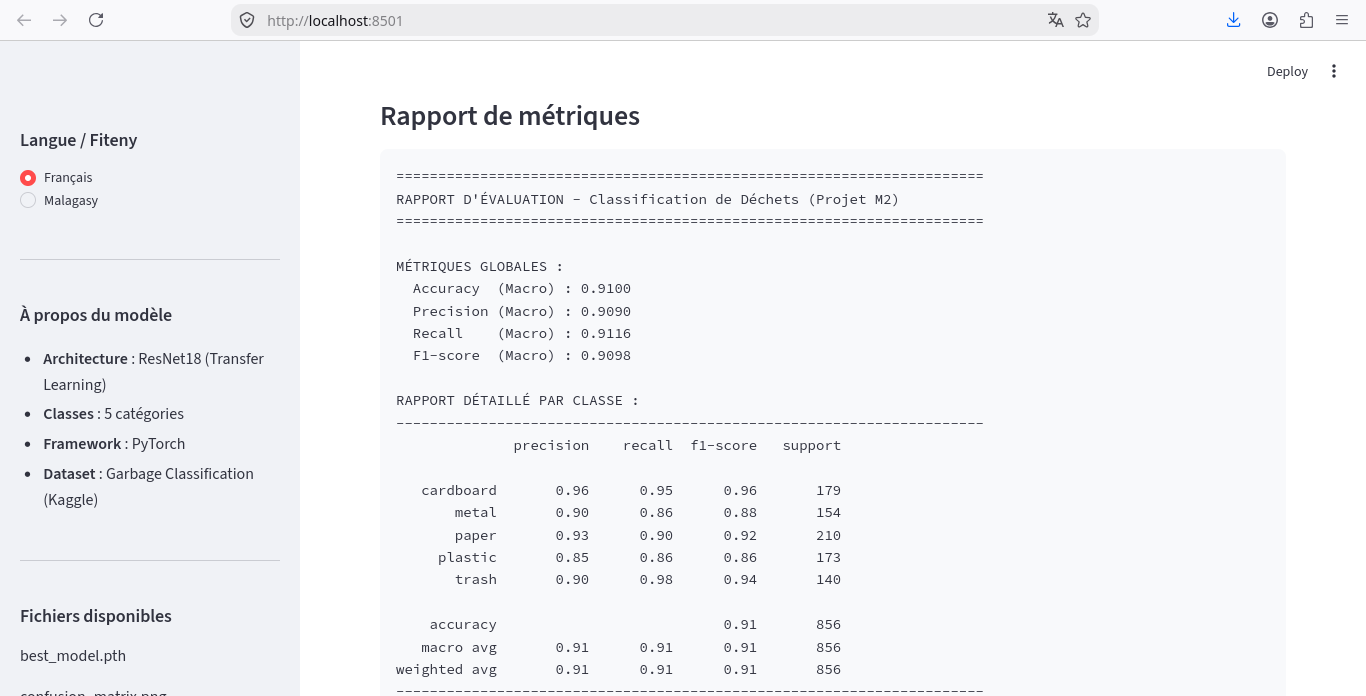
\includegraphics[width=\textwidth]{demo/3.png}
    \caption{Fenêtre d'affichage du rapport de métriques du modèle}
    \label{fig:demo3}
\end{figure}

\begin{figure}[H]
    \centering
    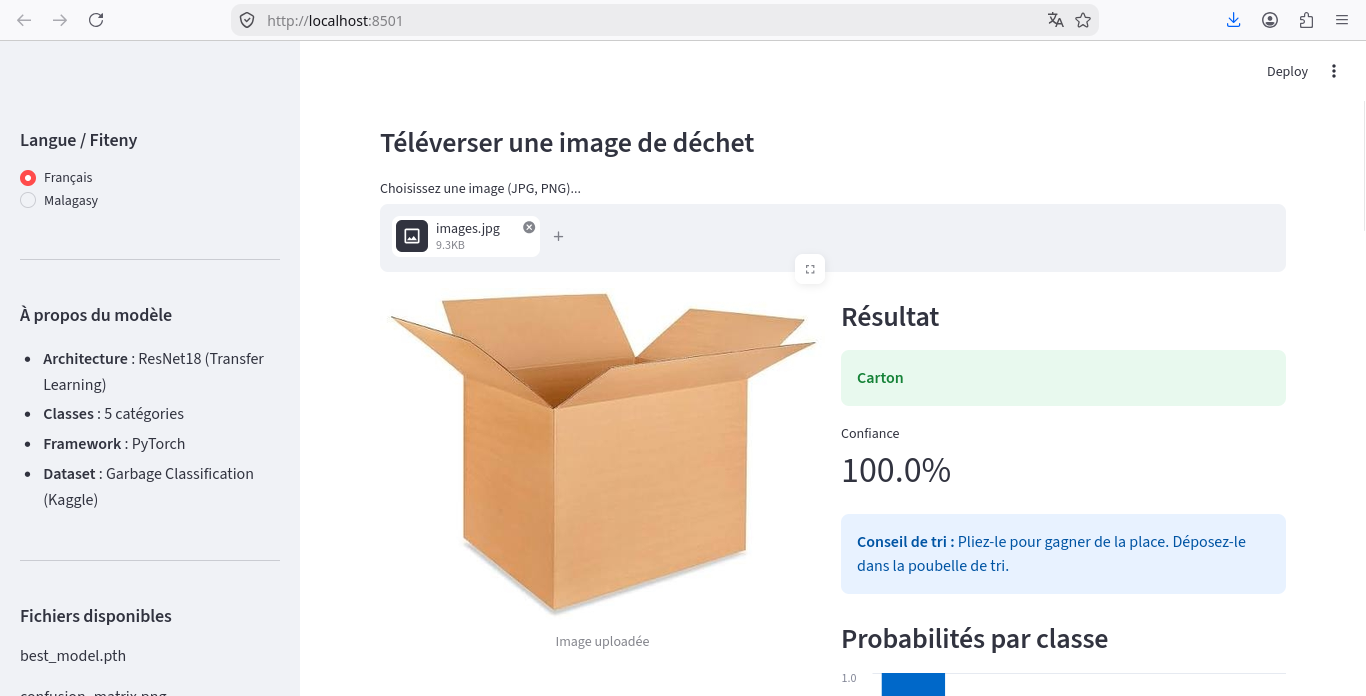
\includegraphics[width=\textwidth]{demo/4.png}
    \caption{Fenêtre des résultats du modèle : courbes d'apprentissage et matrice de confusion}
    \label{fig:demo4}
\end{figure}

\begin{figure}[H]
    \centering
    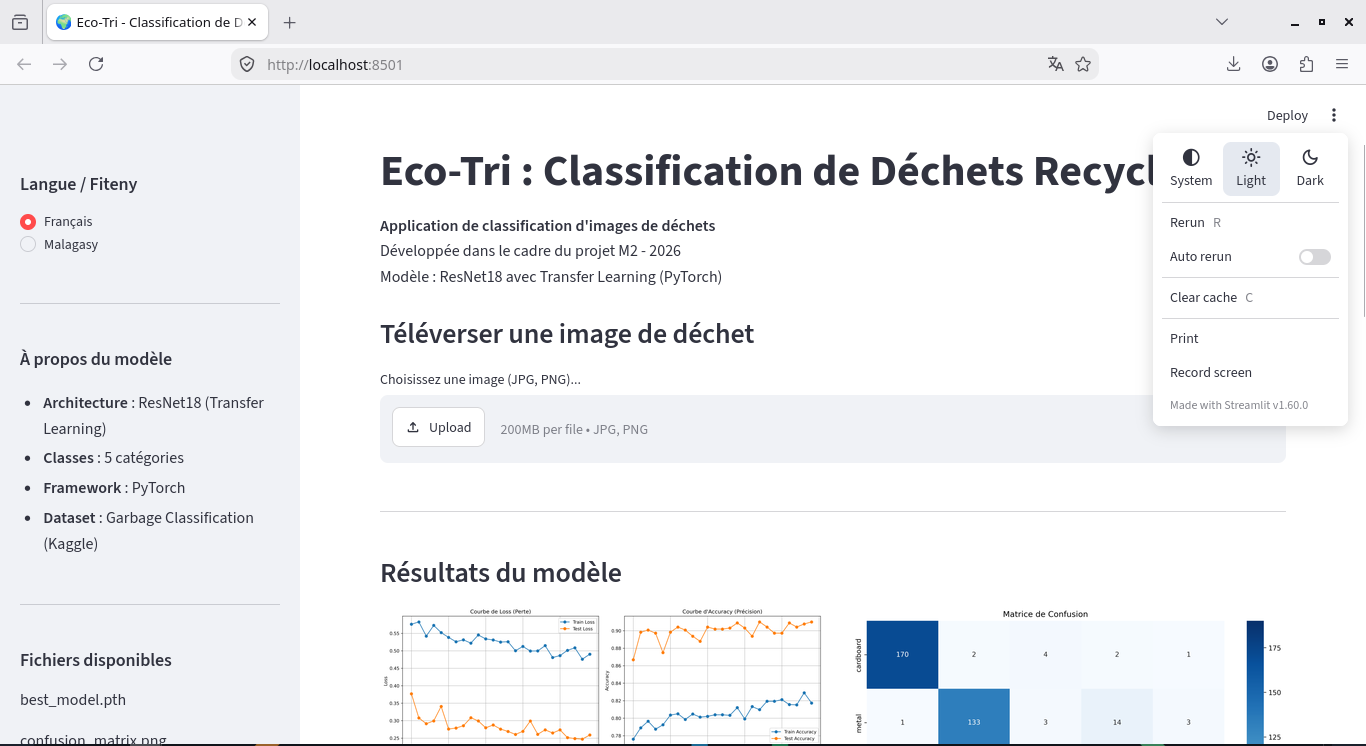
\includegraphics[width=\textwidth]{demo/5.png}
    \caption{Fenêtre des paramètres de l'application : choix de la langue, informations sur le modèle et fichiers disponibles}
    \label{fig:demo5}
\end{figure}

\section{Guide d'Utilisation}
\begin{enumerate}
    \item Lancer l'application : \texttt{streamlit run app/app.py}
    \item Sélectionner la langue (Français / Malagasy) dans la barre latérale.
    \item Téléverser une image de déchet.
    \item Visualiser instantanément le résultat de la classification.
\end{enumerate}

\section{Lien vers le Dépôt Git}
Le code source complet, commenté et documenté, est disponible sur :
\begin{center}
\url{https://github.com/maminiaina-tech/eco_tri.git}
\end{center}

Le dépôt contient :
\begin{itemize}
    \item \texttt{app/} : Code source de l'application (Python).
    \item \texttt{colab/} : Notebook d'entraînement Jupyter.
    \item \texttt{data/} : Documentation du dataset.
    \item \texttt{results/} : Modèle entraîné et résultats.
    \item \texttt{requirements.txt} : Dépendances.
    \item \texttt{README.md} : Documentation complète.
\end{itemize}

% ====================================================================
% CHAPITRE 8 : CONCLUSION ET PERSPECTIVES
% ====================================================================
\chapter{Conclusion et Perspectives}

\section{Conclusion Générale}
Le présent mémoire a permis de concevoir, d'implémenter et d'évaluer un système complet de classification automatique de déchets recyclables, dénommé \textbf{Eco-Tri}, fondé sur les techniques de la vision par ordinateur et du Deep Learning. À l'issue d'une étude bibliographique ayant consolidé les fondements théoriques des réseaux de neurones convolutifs et du transfert d'apprentissage, puis d'une revue de l'état de l'art ayant situé notre démarche parmi les travaux existants, un modèle ResNet18 pré-entraîné sur ImageNet a été adapté par extraction de caractéristiques à la classification de 4~272 images réparties en cinq classes (carton, métal, papier, plastique et déchet non recyclable). Le pipeline d'entraînement, implémenté sous PyTorch et exécuté sur GPU, a permis d'atteindre une exactitude de \textbf{91\,\%} et un F1-score macro de \textbf{0.91} sur le jeu de test, dépassant ainsi l'objectif initial fixé à 90\,\% et confirmant la robustesse de l'approche malgré quelques confusions résiduelles entre classes visuellement proches telles que le plastique et le déchet non recyclable. Au-delà de la dimension scientifique, le projet a donné naissance à une application interactive développée avec Streamlit, dotée d'une interface bilingue français--malgache, qui rend le modèle accessible au grand public et l'accompagne de conseils de tri personnalisés, contribuant ainsi à la sensibilisation aux enjeux du recyclage. Les principales limites identifiées, à savoir le nombre restreint de classes, le léger déséquilibre du jeu de données et l'apparition modérée d'un surapprentissage en fin d'entraînement, ouvrent la voie à des perspectives prometteuses : l'enrichissement du dataset par de nouvelles catégories (verre, organique, électronique), l'exploration d'architectures plus récentes telles qu'EfficientNet ou les Vision Transformers, l'application de techniques d'augmentation avancées (MixUp, CutMix, GANs), le déploiement sur plateformes mobiles via ONNX ou TensorFlow Lite, et l'extension vers la détection d'objets multi-instances avec YOLO. En définitive, Eco-Tri constitue une preuve de concept aboutie démontrant qu'une solution de tri intelligent, à la fois performante, légère et accessible, peut significativement contribuer à une gestion plus durable des déchets et à la réduction de l'empreinte environnementale.

\section{Forces de l'Approche}
\begin{itemize}
    \item Performance élevée (91\%) avec un modèle léger (11M paramètres).
    \item Reproductibilité assurée par le pipeline documenté.
    \item Application accessible avec interface interactive.
    \item Impact sociétal via la sensibilisation au tri sélectif.
\end{itemize}

\section{Limitations}
\begin{itemize}
    \item 5 classes seulement (verre exclu).
    \item Légers déséquilibres dans les données.
    \item Surapprentissage modéré après 20 époques.
\end{itemize}

\section{Perspectives}
\begin{enumerate}
    \item \textbf{Dataset :} Ajouter des classes (verre, organique, électronique), collecter plus d'images.
    \item \textbf{Modèle :} Tester EfficientNet, ConvNeXt, Vision Transformers.
    \item \textbf{Augmentation :} MixUp, CutMix, GANs pour générer des variations.
    \item \textbf{Déploiement mobile :} Conversion ONNX ou TensorFlow Lite pour smartphone.
    \item \textbf{Détection :} Passer de la classification à la détection d'objets (YOLO).
    \item \textbf{Continuous Learning :} Boucle de rétroaction pour amélioration continue.
\end{enumerate}

\begin{thebibliography}{9}

\bibitem{lecun1998}
Y. LeCun, L. Bottou, Y. Bengio et P. Haffner,
\textit{Gradient-Based Learning Applied to Document Recognition},
Proceedings of the IEEE, 86(11):2278-2324, 1998.

\bibitem{he2016deep}
K. He, X. Zhang, S. Ren et J. Sun,
\textit{Deep Residual Learning for Image Recognition},
IEEE Conference on Computer Vision and Pattern Recognition (CVPR), 2016.

\bibitem{kingma2014adam}
D. P. Kingma et J. Ba,
\textit{Adam: A Method for Stochastic Optimization},
International Conference on Learning Representations (ICLR), 2015.

\bibitem{krizhevsky2012}
A. Krizhevsky, I. Sutskever et G. E. Hinton,
\textit{ImageNet Classification with Deep Convolutional Neural Networks},
Advances in Neural Information Processing Systems (NeurIPS), 2012.

\bibitem{deng2009}
J. Deng, W. Dong, R. Socher, L.-J. Li, K. Li et L. Fei-Fei,
\textit{ImageNet: A Large-Scale Hierarchical Image Database},
IEEE Conference on Computer Vision and Pattern Recognition (CVPR), 2009.

\bibitem{mostafa2020}
M. Abla,
\textit{Garbage Classification Dataset},
Kaggle, 2020.
\url{https://www.kaggle.com/datasets/mostafaabla/garbage-classification}

\bibitem{yang2016}
M. Yang et G. Thung,
\textit{Classification of Trash for Recyclability Status},
CS229 Project Report, Stanford University, 2016.

\bibitem{aral2018}
R. A. Aral, S. R. Keskin, M. Kaya et M. Hacıömeroğlu,
\textit{Classification of TrashNet Dataset Based on Deep Learning Models},
IEEE International Conference on Big Data, 2018.

\end{thebibliography}

\appendix

\chapter{Guide d'Installation et d'Exécution}

\section{Prérequis}
\begin{itemize}
    \item Python 3.10 ou supérieur
    \item pip (gestionnaire de paquets)
    \item Git
\end{itemize}

\section{Installation}
\begin{lstlisting}[language=bash, caption={Commandes d'installation}]
# Cloner le depot
git clone https://github.com/maminiaina-tech/eco_tri.git
cd eco-tri

# Installer les dependances
pip install -r requirements.txt

# Lancer l'application
streamlit run app/app.py
\end{lstlisting}

\section{Entraînement du Modèle (Google Colab)}
\begin{enumerate}
    \item Ouvrir \texttt{colab/training.ipynb} sur Google Colab.
    \item Runtime $\rightarrow$ Changer le type $\rightarrow$ GPU T4.
    \item Exécuter toutes les cellules (15-20 min).
    \item Télécharger les fichiers dans \texttt{results/} :
    \begin{itemize}
        \item \texttt{best\_model.pth}
        \item \texttt{training\_curves.png}
        \item \texttt{confusion\_matrix.png}
        \item \texttt{metrics\_report.txt}
    \end{itemize}
\end{enumerate}

\section{Redémarrer l'Application}
\begin{lstlisting}[language=bash]
# Apres avoir place le modele dans results/
streamlit run app/app.py
\end{lstlisting}

\end{document}
